\documentclass{beamer}

\usepackage[utf8]{inputenc}
\usepackage[T1]{fontenc}
\usepackage{tikz}
\usepackage{fontspec}
\usepackage{wrapfig}
\usepackage{float}
\usepackage{amsmath}
\usepackage{varwidth}
\usepackage[font=scriptsize]{caption}

\usetheme{metropolis}
\usetikzlibrary{matrix}
\usetikzlibrary{calc}
\usetikzlibrary{external}
\tikzexternalize[prefix=build/]
\setmainfont[Ligatures=TeX]{Fira Sans}

\title{Pronalazak najkraćeg puta algoritmom A*}

\date{\vspace{1em}Zagreb, 3. lipnja 2019.}

\institute{Fakultet elektrotehnike i računarstva}

\author{Marko Lazarić\\
Voditelj: Doc. dr. sc. Marko Čupić}

\newcommand{\engl}[1]{ (engl. \emph{#1})}
\newcommand{\twocolumns}[2]{
	\begin{columns}
		\begin{column}{0.4\textwidth}
			#1
		\end{column}
		\begin{column}{0.6\textwidth}  %%<--- here
			#2
		\end{column}
	\end{columns}
}
\newcommand{\state}[2]{\textsc{Stanje}(\( #1 \), \( #2 \))}
\newcommand{\visit}[2]{\fill[fill = red] (#1, #2) rectangle ++(1, 1);}
\newcommand{\find}[2]{\fill[fill = green] (#1, #2) rectangle ++(1, 1);}

\newcommand{\actionName}[1]{#1}
\newcommand{\upAction}{\actionName{Gore}}
\newcommand{\downAction}{\actionName{Dolje}}
\newcommand{\leftAction}{\actionName{Lijevo}}
\newcommand{\rightAction}{\actionName{Desno}}

%\setbeameroption{show notes}
%\setbeamertemplate{note page}[plain]
\renewcommand{\figurename}{Slika}

\begin{document}
  \begin{frame}[noframenumbering, plain]
  	\centering
  	\vspace{3em}
  	Seminarski rad
  	\vspace{-5em}
  	
  	\titlepage
  \end{frame}

	\begin{frame}{Motivacija - Razne slagalice}
		\begin{figure}
			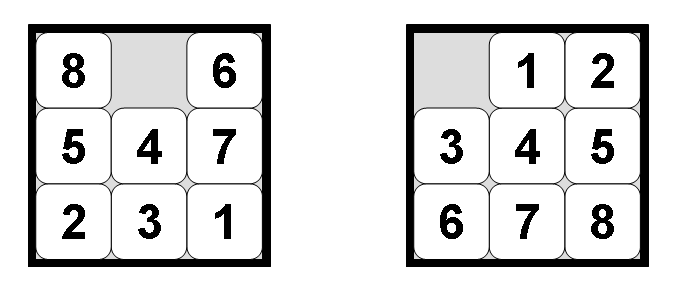
\includegraphics[scale=0.5]{images/8puzzle.png}
			\caption{Slika preuzeta s http://www.aiai.ed.ac.uk/\~{}gwickler/eightpuzzle-uninf.html}
		\end{figure}
	\end{frame}

	\begin{frame}{Motivacija - Rubikova kocka}
		\begin{figure}
			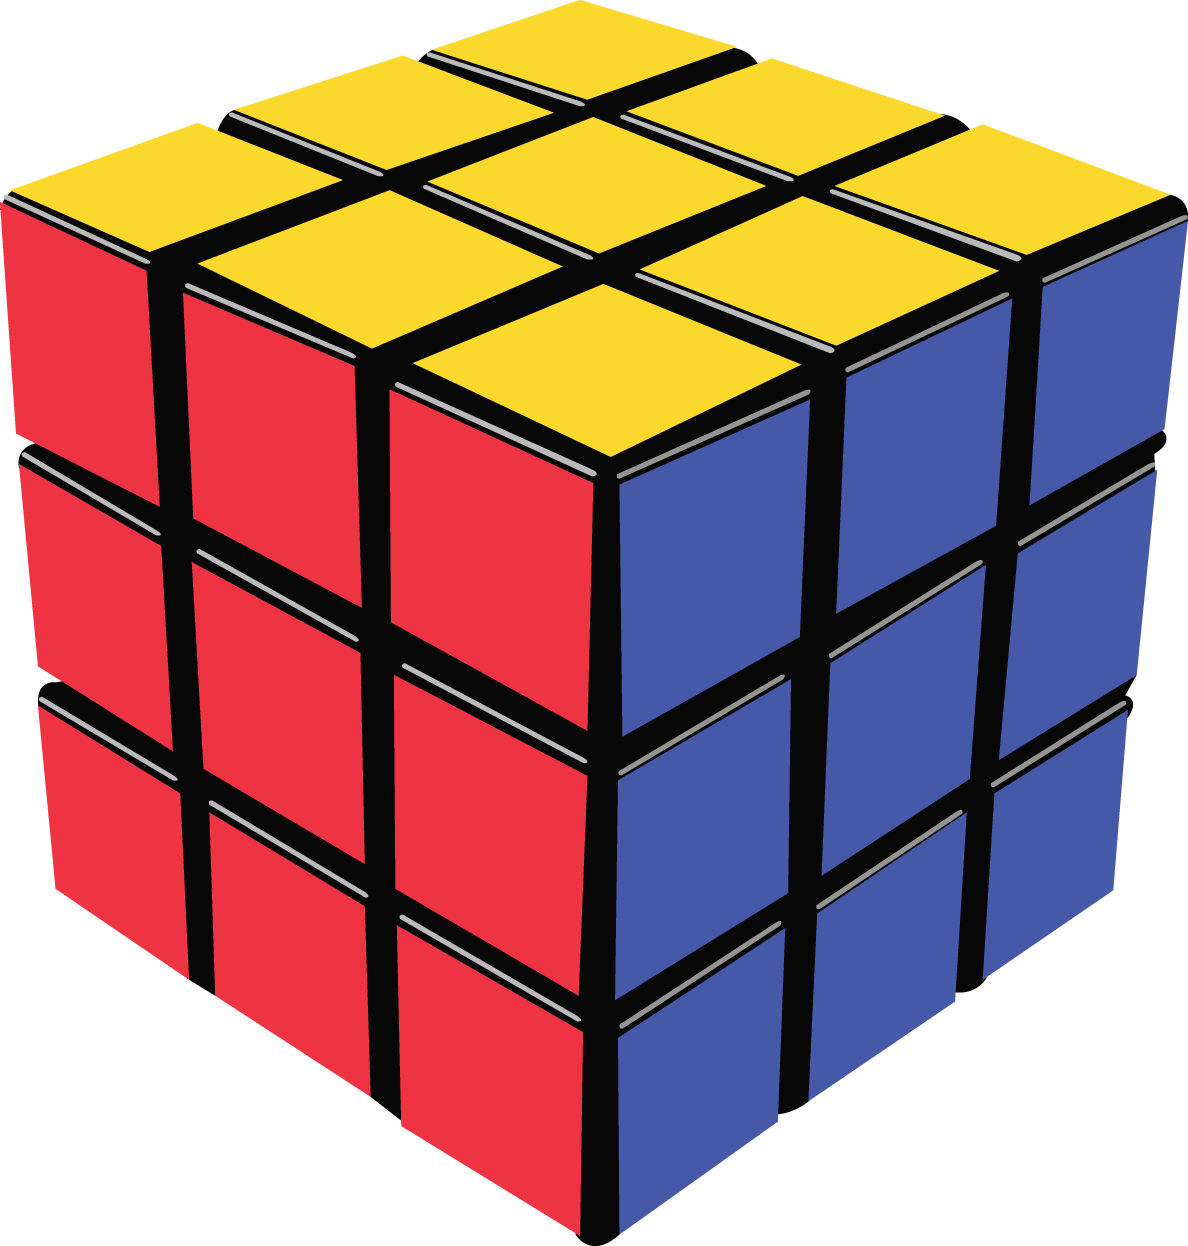
\includegraphics[scale=0.4]{images/rubik_cube.png}
			\caption{Slika preuzeta s http://pngimg.com/imgs/objects/rubik\_cube/}
		\end{figure}
	\end{frame}

	\begin{frame}{Motivacija - Putovanje po Istri}
		\begin{figure}
			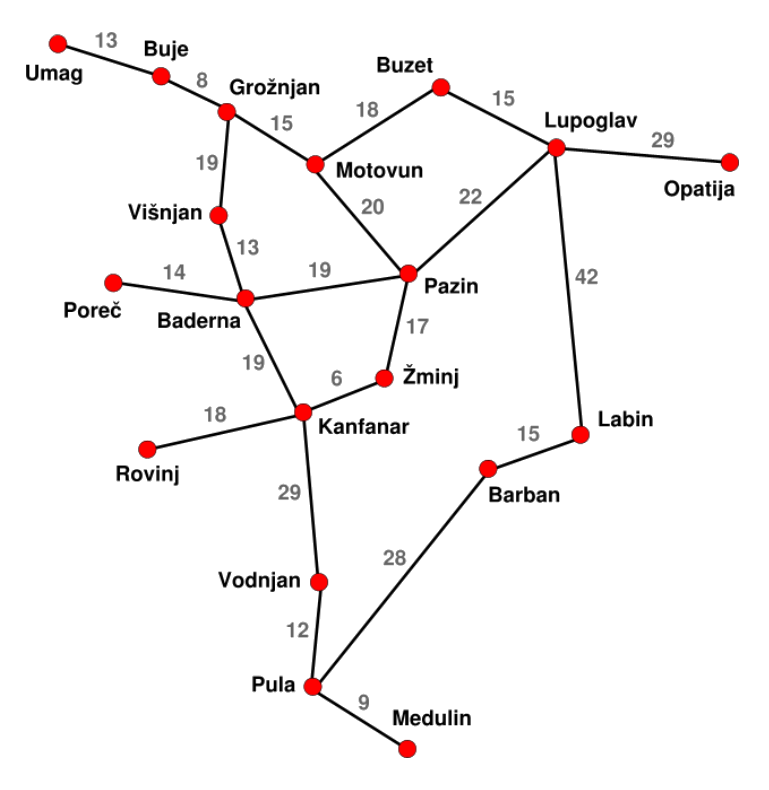
\includegraphics[scale=0.3]{images/istra.png}
			\caption{Slika preuzeta s https://www.fer.unizg.hr/\_download/repository/UI-3-HeuristickoPretrazivanje.pdf}
		\end{figure}
	\end{frame}

  \begin{frame}{Cjelobrojna rešetka}
  	\begin{figure}[h]
  		\centering
  		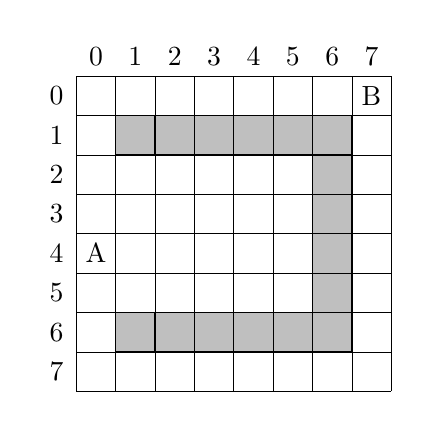
\begin{tikzpicture}
  			\begin{scope}[xshift=0.25cm, yshift=-0.25cm]
	\draw[step=0.5cm,black,very thin] (-2,-2) grid (2,2);
	
	\newcommand\fillSquare[2]{\filldraw[fill=lightgray] (#1 / 2,#2 / 2) rectangle (#1 / 2 + 0.5,#2 / 2 + 0.5)}
	
	
	\foreach \x in {-3,...,2}
	{
		\fillSquare{\x}{-3};
		\fillSquare{\x}{2};
		\fillSquare{2}{\x};
	}
\end{scope}

\matrix[matrix, matrix of nodes, nodes={anchor=center,inner sep=0pt,text width=.5cm,align=center,minimum height=.5cm}, nodes in empty cells]{
& 0 & 1 & 2 & 3 & 4 & 5 & 6 & 7 \\
 0 &   &   &   &   &   &   &   & B \\
	1 &   &   &   &   &   &   &   &   \\
	2 &   &   &   &   &   &   &   &   \\
	3 &   &   &   &   &   &   &   &   \\
	4 & A &   &   &   &   &   &   &   \\
	5 &   &   &   &   &   &   &   &   \\
	6 &   &   &   &   &   &   &   &   \\
	7 &   &   &   &   &   &   &   &   \\};
  		\end{tikzpicture}
  	\end{figure}
  \end{frame}
  
%  \begin{frame}{Prostor stanja - definicija}
%  	\begin{itemize}
%  		\item Graf u kojem vrhovi predstavljaju stanja u problemu, a bridovi prijelaze između stanja
%  		\item Rješavanje problema se svodi na pretraživanje grafa
%  	\end{itemize}
%  \end{frame}
  
  \begin{frame}{Prostor stanja - stanja}
	  \begin{figure}[h]
	  	\centering
	  	\tikzsetnextfilename{states}
	  	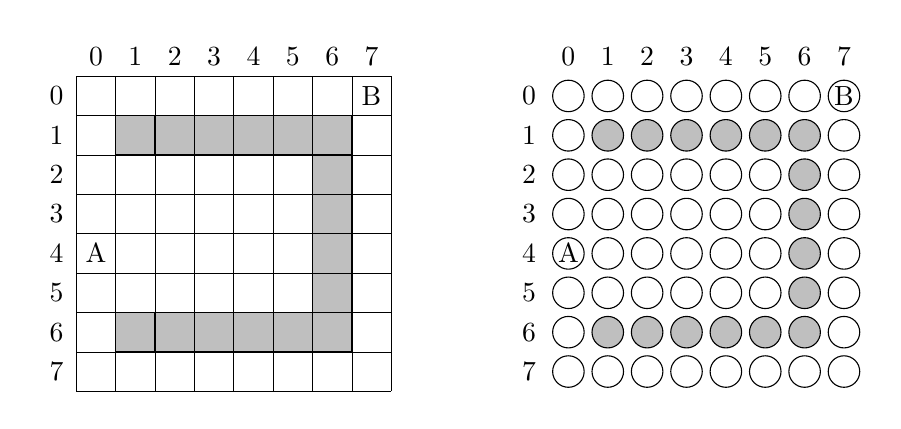
\begin{tikzpicture}
		  	\begin{scope}
		  		\begin{scope}[xshift=0.25cm, yshift=-0.25cm]
	\draw[step=0.5cm,black,very thin] (-2,-2) grid (2,2);
	
	\newcommand\fillSquare[2]{\filldraw[fill=lightgray] (#1 / 2,#2 / 2) rectangle (#1 / 2 + 0.5,#2 / 2 + 0.5)}
	
	
	\foreach \x in {-3,...,2}
	{
		\fillSquare{\x}{-3};
		\fillSquare{\x}{2};
		\fillSquare{2}{\x};
	}
\end{scope}

\matrix[matrix, matrix of nodes, nodes={anchor=center,inner sep=0pt,text width=.5cm,align=center,minimum height=.5cm}, nodes in empty cells]{
& 0 & 1 & 2 & 3 & 4 & 5 & 6 & 7 \\
 0 &   &   &   &   &   &   &   & B \\
	1 &   &   &   &   &   &   &   &   \\
	2 &   &   &   &   &   &   &   &   \\
	3 &   &   &   &   &   &   &   &   \\
	4 & A &   &   &   &   &   &   &   \\
	5 &   &   &   &   &   &   &   &   \\
	6 &   &   &   &   &   &   &   &   \\
	7 &   &   &   &   &   &   &   &   \\};
		  	\end{scope}
		  	
		  	\begin{scope}[xshift=6cm]
		  		\matrix[matrix, matrix of nodes, nodes={anchor=center,inner sep=0pt,text width=.5cm,align=center,minimum height=.5cm}, nodes in empty cells]{
   	& 0 & 1 & 2 & 3 & 4 & 5 & 6 & 7 \\
   	0 &   &   &   &   &   &   &   &   \\
   	1 &   &   &   &   &   &   &   &   \\
   	2 &   &   &   &   &   &   &   &   \\
   	3 &   &   &   &   &   &   &   &   \\
   	4 &   &   &   &   &   &   &   &   \\
   	5 &   &   &   &   &   &   &   &   \\
   	6 &   &   &   &   &   &   &   &   \\
   	7 &   &   &   &   &   &   &   &   \\};
  	
\newcommand\drawNode[4]{\node[circle,draw,inner sep=0pt,minimum size=0.4cm] at (#1 / 2 - 1.5, #2 / 2 - 2)   (#4) {#3};}
\newcommand\drawWallNode[3]{\node[circle,draw,fill=lightgray,inner sep=0pt,minimum size=0.4cm] at (#1 / 2 - 1.5, #2 / 2 - 2)   (#3) {};}

\drawNode{0}{0}{ }{0}
\drawNode{1}{0}{ }{1}
\drawNode{2}{0}{ }{2}
\drawNode{3}{0}{ }{3}
\drawNode{4}{0}{ }{4}
\drawNode{5}{0}{ }{5}
\drawNode{6}{0}{ }{6}
\drawNode{7}{0}{ }{7}
\drawNode{0}{1}{ }{8}
\drawWallNode{1}{1}{9}
\drawWallNode{2}{1}{10}
\drawWallNode{3}{1}{11}
\drawWallNode{4}{1}{12}
\drawWallNode{5}{1}{13}
\drawWallNode{6}{1}{14}
\drawNode{7}{1}{ }{15}
\drawNode{0}{2}{ }{16}
\drawNode{1}{2}{ }{17}
\drawNode{2}{2}{ }{18}
\drawNode{3}{2}{ }{19}
\drawNode{4}{2}{ }{20}
\drawNode{5}{2}{ }{21}
\drawWallNode{6}{2}{22}
\drawNode{7}{2}{ }{23}
\drawNode{0}{3}{A}{24}
\drawNode{1}{3}{ }{25}
\drawNode{2}{3}{ }{26}
\drawNode{3}{3}{ }{27}
\drawNode{4}{3}{ }{28}
\drawNode{5}{3}{ }{29}
\drawWallNode{6}{3}{30}
\drawNode{7}{3}{ }{31}
\drawNode{0}{4}{ }{32}
\drawNode{1}{4}{ }{33}
\drawNode{2}{4}{ }{34}
\drawNode{3}{4}{ }{35}
\drawNode{4}{4}{ }{36}
\drawNode{5}{4}{ }{37}
\drawWallNode{6}{4}{38}
\drawNode{7}{4}{ }{39}
\drawNode{0}{5}{ }{40}
\drawNode{1}{5}{ }{41}
\drawNode{2}{5}{ }{42}
\drawNode{3}{5}{ }{43}
\drawNode{4}{5}{ }{44}
\drawNode{5}{5}{ }{45}
\drawWallNode{6}{5}{46}
\drawNode{7}{5}{ }{47}
\drawNode{0}{6}{ }{48}
\drawWallNode{1}{6}{49}
\drawWallNode{2}{6}{50}
\drawWallNode{3}{6}{51}
\drawWallNode{4}{6}{52}
\drawWallNode{5}{6}{53}
\drawWallNode{6}{6}{54}
\drawNode{7}{6}{ }{55}
\drawNode{0}{7}{ }{56}
\drawNode{1}{7}{ }{57}
\drawNode{2}{7}{ }{58}
\drawNode{3}{7}{ }{59}
\drawNode{4}{7}{ }{60}
\drawNode{5}{7}{ }{61}
\drawNode{6}{7}{ }{62}
\drawNode{7}{7}{B}{63}
		  	\end{scope}
	  	\end{tikzpicture}
	  \end{figure}
  
    \note{Brojni problemi se mogu prikazati grafom u kojem vrhovi predstavljaju stanja, a bridovi prijelaze između tih stanja. Takav graf se naziva prostor stanja. Rješavanje problema se onda svodi na pretraživanje prostora stanja, odnosno pronalazak najkraćeg puta između dva vrha u prostoru stanja. Jednostavan primjer je cjelobrojna rešetka. Svako polje predstavlja jedno stanje, a prijelazi su mogući između svih prolaznih (bijelih) polja. Siva polja predstavljaju zidove. A je početno polje, B je cilj.}
  \end{frame}

	\begin{frame}{Prostor stanja - prijelazi}
		\begin{figure}[h]
			\centering
			\tikzsetnextfilename{space_state}
			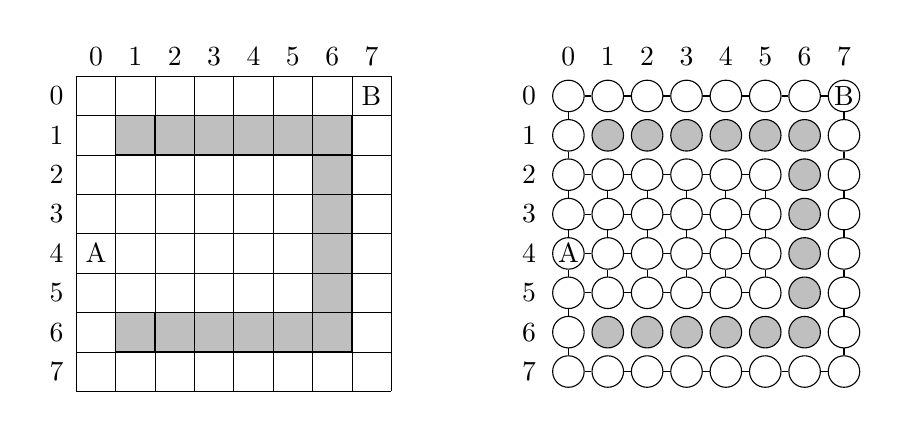
\begin{tikzpicture}
			\begin{scope}
			\begin{scope}[xshift=0.25cm, yshift=-0.25cm]
	\draw[step=0.5cm,black,very thin] (-2,-2) grid (2,2);
	
	\newcommand\fillSquare[2]{\filldraw[fill=lightgray] (#1 / 2,#2 / 2) rectangle (#1 / 2 + 0.5,#2 / 2 + 0.5)}
	
	
	\foreach \x in {-3,...,2}
	{
		\fillSquare{\x}{-3};
		\fillSquare{\x}{2};
		\fillSquare{2}{\x};
	}
\end{scope}

\matrix[matrix, matrix of nodes, nodes={anchor=center,inner sep=0pt,text width=.5cm,align=center,minimum height=.5cm}, nodes in empty cells]{
& 0 & 1 & 2 & 3 & 4 & 5 & 6 & 7 \\
 0 &   &   &   &   &   &   &   & B \\
	1 &   &   &   &   &   &   &   &   \\
	2 &   &   &   &   &   &   &   &   \\
	3 &   &   &   &   &   &   &   &   \\
	4 & A &   &   &   &   &   &   &   \\
	5 &   &   &   &   &   &   &   &   \\
	6 &   &   &   &   &   &   &   &   \\
	7 &   &   &   &   &   &   &   &   \\};
			\end{scope}
			
			\begin{scope}[xshift=6cm]
			\matrix[matrix, matrix of nodes, nodes={anchor=center,inner sep=0pt,text width=.5cm,align=center,minimum height=.5cm}, nodes in empty cells]{
   	& 0 & 1 & 2 & 3 & 4 & 5 & 6 & 7 \\
   	0 &   &   &   &   &   &   &   &   \\
   	1 &   &   &   &   &   &   &   &   \\
   	2 &   &   &   &   &   &   &   &   \\
   	3 &   &   &   &   &   &   &   &   \\
   	4 &   &   &   &   &   &   &   &   \\
   	5 &   &   &   &   &   &   &   &   \\
   	6 &   &   &   &   &   &   &   &   \\
   	7 &   &   &   &   &   &   &   &   \\};
  	
\newcommand\drawNode[4]{\node[circle,draw,inner sep=0pt,minimum size=0.4cm] at (#1 / 2 - 1.5, #2 / 2 - 2)   (#4) {#3};}
\newcommand\drawWallNode[3]{\node[circle,draw,fill=lightgray,inner sep=0pt,minimum size=0.4cm] at (#1 / 2 - 1.5, #2 / 2 - 2)   (#3) {};}

\drawNode{0}{0}{ }{0}
\drawNode{1}{0}{ }{1}
\drawNode{2}{0}{ }{2}
\drawNode{3}{0}{ }{3}
\drawNode{4}{0}{ }{4}
\drawNode{5}{0}{ }{5}
\drawNode{6}{0}{ }{6}
\drawNode{7}{0}{ }{7}
\drawNode{0}{1}{ }{8}
\drawWallNode{1}{1}{9}
\drawWallNode{2}{1}{10}
\drawWallNode{3}{1}{11}
\drawWallNode{4}{1}{12}
\drawWallNode{5}{1}{13}
\drawWallNode{6}{1}{14}
\drawNode{7}{1}{ }{15}
\drawNode{0}{2}{ }{16}
\drawNode{1}{2}{ }{17}
\drawNode{2}{2}{ }{18}
\drawNode{3}{2}{ }{19}
\drawNode{4}{2}{ }{20}
\drawNode{5}{2}{ }{21}
\drawWallNode{6}{2}{22}
\drawNode{7}{2}{ }{23}
\drawNode{0}{3}{A}{24}
\drawNode{1}{3}{ }{25}
\drawNode{2}{3}{ }{26}
\drawNode{3}{3}{ }{27}
\drawNode{4}{3}{ }{28}
\drawNode{5}{3}{ }{29}
\drawWallNode{6}{3}{30}
\drawNode{7}{3}{ }{31}
\drawNode{0}{4}{ }{32}
\drawNode{1}{4}{ }{33}
\drawNode{2}{4}{ }{34}
\drawNode{3}{4}{ }{35}
\drawNode{4}{4}{ }{36}
\drawNode{5}{4}{ }{37}
\drawWallNode{6}{4}{38}
\drawNode{7}{4}{ }{39}
\drawNode{0}{5}{ }{40}
\drawNode{1}{5}{ }{41}
\drawNode{2}{5}{ }{42}
\drawNode{3}{5}{ }{43}
\drawNode{4}{5}{ }{44}
\drawNode{5}{5}{ }{45}
\drawWallNode{6}{5}{46}
\drawNode{7}{5}{ }{47}
\drawNode{0}{6}{ }{48}
\drawWallNode{1}{6}{49}
\drawWallNode{2}{6}{50}
\drawWallNode{3}{6}{51}
\drawWallNode{4}{6}{52}
\drawWallNode{5}{6}{53}
\drawWallNode{6}{6}{54}
\drawNode{7}{6}{ }{55}
\drawNode{0}{7}{ }{56}
\drawNode{1}{7}{ }{57}
\drawNode{2}{7}{ }{58}
\drawNode{3}{7}{ }{59}
\drawNode{4}{7}{ }{60}
\drawNode{5}{7}{ }{61}
\drawNode{6}{7}{ }{62}
\drawNode{7}{7}{B}{63}
\draw[] (0) -- (8);
\draw[] (0) -- (1);
\draw[] (1) -- (2);
\draw[] (1) -- (0);
\draw[] (2) -- (3);
\draw[] (2) -- (1);
\draw[] (3) -- (4);
\draw[] (3) -- (2);
\draw[] (4) -- (5);
\draw[] (4) -- (3);
\draw[] (5) -- (6);
\draw[] (5) -- (4);
\draw[] (6) -- (7);
\draw[] (6) -- (5);
\draw[] (7) -- (15);
\draw[] (7) -- (6);
\draw[] (8) -- (16);
\draw[] (8) -- (0);
\draw[] (15) -- (23);
\draw[] (15) -- (7);
\draw[] (16) -- (24);
\draw[] (16) -- (8);
\draw[] (16) -- (17);
\draw[] (17) -- (25);
\draw[] (17) -- (18);
\draw[] (17) -- (16);
\draw[] (18) -- (26);
\draw[] (18) -- (19);
\draw[] (18) -- (17);
\draw[] (19) -- (27);
\draw[] (19) -- (20);
\draw[] (19) -- (18);
\draw[] (20) -- (28);
\draw[] (20) -- (21);
\draw[] (20) -- (19);
\draw[] (21) -- (29);
\draw[] (21) -- (20);
\draw[] (23) -- (31);
\draw[] (23) -- (15);
\draw[] (24) -- (32);
\draw[] (24) -- (16);
\draw[] (24) -- (25);
\draw[] (25) -- (33);
\draw[] (25) -- (17);
\draw[] (25) -- (26);
\draw[] (25) -- (24);
\draw[] (26) -- (34);
\draw[] (26) -- (18);
\draw[] (26) -- (27);
\draw[] (26) -- (25);
\draw[] (27) -- (35);
\draw[] (27) -- (19);
\draw[] (27) -- (28);
\draw[] (27) -- (26);
\draw[] (28) -- (36);
\draw[] (28) -- (20);
\draw[] (28) -- (29);
\draw[] (28) -- (27);
\draw[] (29) -- (37);
\draw[] (29) -- (21);
\draw[] (29) -- (28);
\draw[] (31) -- (39);
\draw[] (31) -- (23);
\draw[] (32) -- (40);
\draw[] (32) -- (24);
\draw[] (32) -- (33);
\draw[] (33) -- (41);
\draw[] (33) -- (25);
\draw[] (33) -- (34);
\draw[] (33) -- (32);
\draw[] (34) -- (42);
\draw[] (34) -- (26);
\draw[] (34) -- (35);
\draw[] (34) -- (33);
\draw[] (35) -- (43);
\draw[] (35) -- (27);
\draw[] (35) -- (36);
\draw[] (35) -- (34);
\draw[] (36) -- (44);
\draw[] (36) -- (28);
\draw[] (36) -- (37);
\draw[] (36) -- (35);
\draw[] (37) -- (45);
\draw[] (37) -- (29);
\draw[] (37) -- (36);
\draw[] (39) -- (47);
\draw[] (39) -- (31);
\draw[] (40) -- (48);
\draw[] (40) -- (32);
\draw[] (40) -- (41);
\draw[] (41) -- (33);
\draw[] (41) -- (42);
\draw[] (41) -- (40);
\draw[] (42) -- (34);
\draw[] (42) -- (43);
\draw[] (42) -- (41);
\draw[] (43) -- (35);
\draw[] (43) -- (44);
\draw[] (43) -- (42);
\draw[] (44) -- (36);
\draw[] (44) -- (45);
\draw[] (44) -- (43);
\draw[] (45) -- (37);
\draw[] (45) -- (44);
\draw[] (47) -- (55);
\draw[] (47) -- (39);
\draw[] (48) -- (56);
\draw[] (48) -- (40);
\draw[] (55) -- (63);
\draw[] (55) -- (47);
\draw[] (56) -- (48);
\draw[] (56) -- (57);
\draw[] (57) -- (58);
\draw[] (57) -- (56);
\draw[] (58) -- (59);
\draw[] (58) -- (57);
\draw[] (59) -- (60);
\draw[] (59) -- (58);
\draw[] (60) -- (61);
\draw[] (60) -- (59);
\draw[] (61) -- (62);
\draw[] (61) -- (60);
\draw[] (62) -- (63);
\draw[] (62) -- (61);
\draw[] (63) -- (55);
\draw[] (63) -- (62);
		
			
			
			\end{scope}
			\end{tikzpicture}
		\end{figure}
	\end{frame}

	\begin{frame}[fragile]{Općenit algoritam pretraživanja}
		\begin{figure}
			\centering
			\begin{varwidth}{\linewidth}
				\begin{verbatim}
fronta = prioritetni red 
ubaci u frontu početno stanje i cijenu 0

dok fronta nije prazna
    uzmi prvo stanje i cijenu iz fronte
    obradi to stanje i cijenu
kraj\end{verbatim}
			\end{varwidth}
		\end{figure}
	\end{frame}

	\newcommand{\algoritamFrame}[1]{
		\begin{frame}{Općenit algoritam pretraživanja}
			\centering
			
			\tikzsetnextfilename{algoritam#1}
			\begin{tikzpicture}
				\input{figures/basic#1.tex}
			\end{tikzpicture}
	\end{frame}}

	\algoritamFrame{0}
	\algoritamFrame{1}
	\algoritamFrame{2}
	\algoritamFrame{3}
	\algoritamFrame{4}

	\begin{frame}{Evaluacijska funkcija}
		\begin{itemize}
			\item Evaluacijska funkcija \( f(n) \) svakom stanju \( n \) pridodaje numeričku vrijednost koja predstavlja prioritet pri pretraživanju
			\item Manja vrijednost funkcije predstavlja veći prioritet, odnosno manju "cijenu" 
		\end{itemize}
	\end{frame}

	  \begin{frame}{Pomoćne funkcije}
		\begin{itemize}
			\item \emph{Cijena puta} (\( g(n) \)) predstavlja \textbf{izračunatu} cijenu puta od početnog stanja do stanja \( n \)\\[3em]
			\item \emph{Heuristička funkcija} (\( h(n) \)) predstavlja \textbf{aproksimaciju} najmanje cijene puta od stanja \( n \) do cilja
		\end{itemize}
		\note{Dodatne informacije o problemu ugrađujemo u heurističku funkciju. Heuristička funckija svakom stanju pridodaju numeričku vrijednost koja predstavlja minimalnu cijenu puta od tog stanja do cilja.}
	\end{frame}
	
	\begin{frame}{Heuristička funkcija - primjer}
		\twocolumns{
			\tikzsetnextfilename{heuristic}
			\begin{figure}[H]
				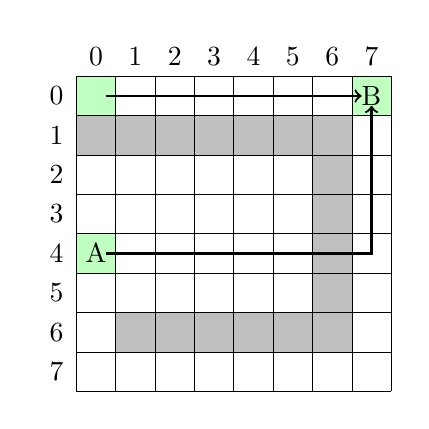
\begin{tikzpicture}
				\begin{scope}[xshift=-1.75cm, yshift=1.75cm, xscale=0.5, yscale=0.5]
	\fill[fill = lightgray] (0, -1) 
	  -- ++(7, 0) 
	  -- ++(0, -6) 
	  -- ++(-6, 0) 
	  -- ++(0, 1) 
	  -- ++(5, 0) 
	  -- ++(0, 4) 
	  -- ++(-6, 0) 
	  -- cycle;
	  
	\fill[fill = green!25] (7, -1) -- ++(1, 0) -- ++(0, 1) -- ++(-1, 0) -- cycle;
	
	\fill[fill = green!25] (0, -1) -- ++(1, 0) -- ++(0, 1) -- ++(-1, 0) -- cycle;
	
	\fill[fill = green!25] (0, -5) -- ++(1, 0) -- ++(0, 1) -- ++(-1, 0) -- cycle;
\end{scope}

\begin{scope}[xshift=0.25cm, yshift=-0.25cm]
	\draw[step=0.5cm,black,very thin] (-2,-2) grid (2,2);
\end{scope}

\matrix[matrix, matrix of nodes, nodes={anchor=center,inner sep=0pt,text width=.5cm,align=center,minimum height=.5cm}, nodes in empty cells]{
	& 0 & 1 & 2 & 3 & 4 & 5 & 6 & 7 \\
	0 &   &   &   &   &   &   &   & B \\
	1 &   &   &   &   &   &   &   &   \\
	2 &   &   &   &   &   &   &   &   \\
	3 &   &   &   &   &   &   &   &   \\
	4 & A &   &   &   &   &   &   &   \\
	5 &   &   &   &   &   &   &   &   \\
	6 &   &   &   &   &   &   &   &   \\
	7 &   &   &   &   &   &   &   &   \\};

\begin{scope}[xshift=-1.75cm, yshift=1.75cm, xscale=0.5, yscale=0.5]
	\draw [->, thick] (0.75, -0.5) -- ++(6.5, 0);
	\draw [->, thick] (0.75, -4.5) -- ++(6.75, 0) -- ++(0, 3.75);
\end{scope}
				\end{tikzpicture}
			\end{figure}
		}{
			\begin{itemize}
				\item Jednostavna heuristika za cjelobrojnu rešetku je Manhattan udaljenost između stanja \\[0.5cm]
			\end{itemize}
			\[ h(\text{\state{x}{y}}) = |x - x_B| + |y - y_B| \]
			\[ h(\text{\state{0}{0}}) = 7 \]
			\[ h(\text{\state{4}{0}}) = 11 \]
		}
		\note{Primjer jednostavne heurističke funkcije za cjelobrojnu rešetku je Manhattan udaljenost između tog stanja i cilja. Primijetimo da je to ujedno i najmanji mogući broj poteza za prijelaz od tog stanja do cilja. Također primijetimo da takav put ne postoji nužno, npr. za stanje 4, 0.}
	\end{frame}

  \begin{frame}{Algoritmi pretraživanja prostora stanja}
    \begin{itemize}
    	\item Naivni (neinformirani) algoritmi
    	\begin{itemize}
    		\item Pretraživanje u širinu 
    		\item Pretraživanje u dubinu 
    		\item Pretraživanje s jednolikom cijenom 
    	\end{itemize}
    	\item Informirani algoritmi
    	\begin{itemize}
    		\item Pretraživanje "prvi najbolji" 
    		\item Algoritam A*
    	\end{itemize}
    \end{itemize}

	\note{Algoritmi pretraživanja prostora stanja se dijele u dvije kategorije: naivni i informirani. Naivni ili neinformirani algoritmi ne koriste dodatne informacije o problemu, nego pretražuju prostor stanja kao običan graf. Oni su generalniji jer ne ovise o problemu koji rješavaju, ali imaju veću vremensku i prostornu složenost jer pretražuju više stanja. Primjeri takvih algoritama su pretraživanje u širinu, pretraživanje u dubinu i pretraživanje s jednolikom cijenom.
	
Informirani algoritmi koriste dodatne informacije o problemu kako bi smanjili dio prostora stanja kojeg trebaju pretražiti. Imaju manju vremensku i prostornu složenost od naivnih jer pretražuju manje stanja, ali su specifični za pojedini problem u jednoj komponenti. Primjeri takvih algoritama su pretraživanje prvi najbolji i algoritam A*.}
  \end{frame}

%  \begin{frame}{Definicija problema}
%    \begin{itemize}
%    	\item Početno stanje
%    	\item Akcije
%    	\item Model prijelaza
%    	\item Provjera rješenja
%    	\item Trošak prijelaza između stanja
%    \end{itemize}
%
%	\note{Takvi problemi se mogu definirati pomoću 5 komponenti: početno stanje, akcije, model prijelaza, provjera rješenja i trošak prijelaza između stanja. Objasnit ću te komponente na primjeru cjelobrojne rešetke.}
%  \end{frame}
%
%  \begin{frame}{Početno stanje}	
%	\begin{figure}[H]
%  		\begin{tikzpicture}
%  		\begin{scope}[xshift=-1.75cm, yshift=1.75cm, xscale=0.5, yscale=0.5]
	\fill[fill = lightgray] (1, -1) 
	  -- ++(6, 0) 
	  -- ++(0, -6) 
	  -- ++(-6, 0) 
	  -- ++(0, 1) 
	  -- ++(5, 0) 
	  -- ++(0, 4) 
	  -- ++(-5, 0) 
	  -- cycle;
	  
	\fill[fill = green!25] (0, -5) -- ++(1, 0) -- ++(0, 1) -- ++(-1, 0) -- cycle;
	
\end{scope}

\begin{scope}[xshift=0.25cm, yshift=-0.25cm]
	\draw[step=0.5cm,black,very thin] (-2,-2) grid (2,2);
\end{scope}

\matrix[matrix, matrix of nodes, nodes={anchor=center,inner sep=0pt,text width=.5cm,align=center,minimum height=.5cm}, nodes in empty cells]{
	& 0 & 1 & 2 & 3 & 4 & 5 & 6 & 7 \\
	0 &   &   &   &   &   &   &   & B \\
	1 &   &   &   &   &   &   &   &   \\
	2 &   &   &   &   &   &   &   &   \\
	3 &   &   &   &   &   &   &   &   \\
	4 & A &   &   &   &   &   &   &   \\
	5 &   &   &   &   &   &   &   &   \\
	6 &   &   &   &   &   &   &   &   \\
	7 &   &   &   &   &   &   &   &   \\};
%  		\end{tikzpicture}
%	\end{figure}
%
%	\note{Početno stanje \engl{inital state} je stanje u kojem počinje pretraživanje. U slučaju cjelobrojne rešetke, to je stanje koje sadrži "A" obojano zelenom bojom.}
%  \end{frame}
%
%  \begin{frame}{Akcije}
%   	\begin{figure}[H]
%   		\begin{tikzpicture}
%   		\begin{scope}[xshift=-1.75cm, yshift=1.75cm, xscale=0.5, yscale=0.5]
	\fill[fill = lightgray] (1, -1) 
	  -- ++(6, 0) 
	  -- ++(0, -6) 
	  -- ++(-6, 0) 
	  -- ++(0, 1) 
	  -- ++(5, 0) 
	  -- ++(0, 4) 
	  -- ++(-5, 0) 
	  -- cycle;
	  
	  \fill[fill = green!25] (3, -5) -- ++(1, 0) -- ++(0, 1) -- ++(-1, 0) -- cycle;
	  \fill[fill = green!25] (3, -1) -- ++(1, 0) -- ++(0, 1) -- ++(-1, 0) -- cycle;
	  \fill[fill = green!25] (0, -7) -- ++(1, 0) -- ++(0, 1) -- ++(-1, 0) -- cycle;
\end{scope}

\begin{scope}[xshift=0.25cm, yshift=-0.25cm]
	\draw[step=0.5cm,black,very thin] (-2,-2) grid (2,2);
\end{scope}

\matrix[matrix, matrix of nodes, nodes={anchor=center,inner sep=0pt,text width=.5cm,align=center,minimum height=.5cm}, nodes in empty cells]{
	& 0 & 1 & 2 & 3 & 4 & 5 & 6 & 7 \\
	0 &   &   &   &   &   &   &   & B \\
	1 &   &   &   &   &   &   &   &   \\
	2 &   &   &   &   &   &   &   &   \\
	3 &   &   &   &   &   &   &   &   \\
	4 & A &   &   &   &   &   &   &   \\
	5 &   &   &   &   &   &   &   &   \\
	6 &   &   &   &   &   &   &   &   \\
	7 &   &   &   &   &   &   &   &   \\};

\begin{scope}[xshift=-1.75cm, yshift=1.75cm, xscale=0.5, yscale=0.5]
	\draw [->, thick] (3.25, -4.5) -- ++(-0.5, 0);
	\draw [->, thick] (3.75, -4.5) -- ++(0.5, 0);
	\draw [->, thick] (3.5, -4.75) -- ++(0, -0.5);
	\draw [->, thick] (3.5, -4.25) -- ++(0, 0.5);
	
	\draw [->, thick] (0.5, -6.75) -- ++(0, -0.5);
	\draw [->, thick] (0.5, -6.25) -- ++(0, 0.5);
	
	\draw [->, thick] (3.25, -0.5) -- ++(-0.5, 0);
	\draw [->, thick] (3.75, -0.5) -- ++(0.5, 0);
\end{scope}
%   		\end{tikzpicture}
%   	\end{figure}
%
%    \note{Akcije \engl{actions} je popis mogućih akcija koje je moguće poduzeti iz trenutnog stanja. U slučaju cjelobrojne rešetke, moguće akcije su pomakni se gore, dolje, lijevo i desno kao što je prikazano na slici.}
%  \end{frame}
%
%  \begin{frame}{Model prijelaza}
%    \begin{itemize}
%    	\item \emph{Model prijelaza} \engl{transition model} opisuje moguće akcije i prijelaze između stanja
%    	\item U slučaju cjelobrojne rešetke, model prijelaza je:
%    	\\[1em]
%    	\begin{tabular}{lcl}
%    		\textsc{Rezultat}(\state{x}{y}, \upAction) &=& \state{x}{y - 1} \\
%    		\textsc{Rezultat}(\state{x}{y}, \downAction) &=& \state{x}{y + 1} \\
%    		\textsc{Rezultat}(\state{x}{y}, \leftAction) &=& \state{x - 1}{y} \\
%    		\textsc{Rezultat}(\state{x}{y}, \rightAction) &=& \state{x + 1}{y}
%    	\end{tabular}
%    	%\begin{itemize}
%    	%	\item \textsc{Rezultat}(Stanje(x, y), Gore) = Stanje(x, y - 1)
%    	%	\item \textsc{Rezultat}(Stanje(x, y), Dolje) = Stanje(x, y + 1)
%    	%	\item \textsc{Rezultat}(Stanje(x, y), Lijevo) = Stanje(x - 1, y)
%    	%	\item \textsc{Rezultat}(Stanje(x, y), Desno) = Stanje(x + 1, y)
%    	%\end{itemize}
%    \end{itemize}
%  \end{frame}
%
%  \begin{frame}{Provjera rješenja}
%   	\begin{figure}[H]
%		\begin{tikzpicture}
%			\begin{scope}[xshift=-1.75cm, yshift=1.75cm, xscale=0.5, yscale=0.5]
	\fill[fill = lightgray] (1, -1) 
	  -- ++(6, 0) 
	  -- ++(0, -6) 
	  -- ++(-6, 0) 
	  -- ++(0, 1) 
	  -- ++(5, 0) 
	  -- ++(0, 4) 
	  -- ++(-5, 0) 
	  -- cycle;
	  
	\fill[fill = green!25] (7, -1) -- ++(1, 0) -- ++(0, 1) -- ++(-1, 0) -- cycle;
	
\end{scope}

\begin{scope}[xshift=0.25cm, yshift=-0.25cm]
	\draw[step=0.5cm,black,very thin] (-2,-2) grid (2,2);
\end{scope}

\matrix[matrix, matrix of nodes, nodes={anchor=center,inner sep=0pt,text width=.5cm,align=center,minimum height=.5cm}, nodes in empty cells]{
	& 0 & 1 & 2 & 3 & 4 & 5 & 6 & 7 \\
	0 &   &   &   &   &   &   &   & B \\
	1 &   &   &   &   &   &   &   &   \\
	2 &   &   &   &   &   &   &   &   \\
	3 &   &   &   &   &   &   &   &   \\
	4 & A &   &   &   &   &   &   &   \\
	5 &   &   &   &   &   &   &   &   \\
	6 &   &   &   &   &   &   &   &   \\
	7 &   &   &   &   &   &   &   &   \\};
%		\end{tikzpicture}
%	\end{figure}
%
%	\note{Provjera rješenja \engl{goal test} provjerava je li određeno stanje rješenje. Primijetimo da možemo imati više stanja koje predstavljaju rješenje, no ovdje ćemo se ograničiti na jedno. U slučaju cjelobrojne rešetko, rješenje je stanje koje sadrži "B" obojano zelenom bojom.}
%  \end{frame}
%
%  \begin{frame}{Trošak prijelaza između stanja}
%	\begin{itemize}
%      \item \emph{Trošak prijelaza} \engl{step cost} je funkcija koja određuje trošak prijelaza iz stanja \( s \) u stanje \( s' \) akcijom \( a \)
%      \item Označava se \( c(s, a, s') \)
%	  \item U slučaju cjelobrojne rešetke, trošak prijelaza je \( 1 \) za svako susjedno polje (osim zidova)
%    \end{itemize}
%  \end{frame}

%  \begin{frame}{Optimističnost i konzistentnost}
%  	\begin{itemize}
%  		\item Heuristika \( h(n) \) je \emph{optimistična} ili \emph{dopustiva} ako i samo ako nikada ne precjenjuje, odnosno nikada nije veća od prave cijene do cilja \\[3em]
%  		\item Heuristika \( h(n) \) je \emph{konzistentna} ili \emph{monotona} ako i samo ako za svako stanje \( s \) i svaki njegov sljedbenik \( s' \) vrijedi \( h(s) \leq h(s') + c \) gdje je \( c \) trošak prijelaza iz stanja \( s \) u \( s' \)
%  	\end{itemize}
%  \end{frame}


	
	\newcommand{\ucsFrame}[1]{
		\begin{frame}{Pretraživanje s jednolikom cijenom}
			\centering
			\( f(n) = g(n) \)
			
			\tikzsetnextfilename{ucs#1}
			\begin{tikzpicture}
				\input{figures/ucs#1.tex}
			\end{tikzpicture}
		\end{frame}}
	
	
	
	\ucsFrame{0}
	\ucsFrame{1}
	\ucsFrame{2}
	\ucsFrame{3}
	\ucsFrame{4}
	\ucsFrame{5}
	\ucsFrame{6}
	\ucsFrame{7}
	\ucsFrame{8}
	\ucsFrame{9}
	\ucsFrame{10}
	\ucsFrame{11}
	
	\newcommand{\gbfsFrame}[1]{
		\begin{frame}{Pretraživanje "prvi najbolji"}
			\centering
			\( f(n) = h(n) \)
			
			\tikzsetnextfilename{gbfs#1}
			\begin{tikzpicture}
				\input{figures/gbfs#1.tex}
			\end{tikzpicture}
		\end{frame}}
	
	\gbfsFrame{0}
	\gbfsFrame{1}
	\gbfsFrame{2}
	\gbfsFrame{3}
	\gbfsFrame{4}
	\gbfsFrame{5}
	\gbfsFrame{6}
	\gbfsFrame{7}
	\gbfsFrame{8}
	\gbfsFrame{9}
	\gbfsFrame{10}
	\gbfsFrame{11}
	\gbfsFrame{12}
	\gbfsFrame{13}
	\gbfsFrame{14}
	\gbfsFrame{15}
	
	\newcommand{\astarFrame}[1]{
		\begin{frame}{Algoritam A*}
			\centering
			\( f(n) = g(n) + h(n) \)
			
			\tikzsetnextfilename{astar#1}
			\begin{tikzpicture}
				\input{figures/astar#1.tex}
			\end{tikzpicture}
		\end{frame}}
	
	\astarFrame{0}
	\astarFrame{1}
	\astarFrame{2}
	\astarFrame{3}
	\astarFrame{4}
	\astarFrame{5}
	\astarFrame{6}
	\astarFrame{7}
	\astarFrame{8}
	\astarFrame{9}
	\astarFrame{10}
	\astarFrame{11}
	\astarFrame{12}
	\astarFrame{13}
	\astarFrame{14}
	\astarFrame{15}
	\astarFrame{16}

  

  \section{Demonstracija programa}
  
  \begin{frame}[plain]
  	\section{Hvala na pažnji!}
  	\usebeamerfont{frametitle}
  	\hspace{15em}Pitanja?
  \end{frame}
  
\end{document}